%% Template for English Papers
%%%%%%%%%%%%%%%%%%%%%%%%%%%%%%%%%%%%%%%%%%%%%%%%%%%%%%%%%%%%%%%%%%%%%%%%%%%%%%%
 \documentclass[english]{jpnsecart}                   % English Original Paper

%% For JPNSEC office %%%%%%%%%%%%%%%%%%%%%%%%%%%%%%%%%%%%%%%%%%%%%%%%%%%%%%%%%%
% You don't need to modify them. 
\received{2010}{8}{1}
\stuffincharge{XX\hspace{0.5zh} XX}
\setcounter{page}{1}
%\setcounter{volpage}{1}
\Vol{1}
\No{1}

%% CAUSION for amsmath package users %%%%%%%%%%%%%%%%%%%%%%%%%%%%%%%%%%%%%%%%%%
% \usepackpage{amsmath}
% equation No. should be reffered by the \eqref, not \ref
% specify the "fleqn" as the option of documentclass command
% ex. \documentclass[technicalpaper,fleqn]{jpnsecart}
%\usepackage{evocomp}
\usepackage{fancyhdr}
\usepackage{graphicx}
%\addcontentsline{toc}{chapter}{Bibliography}
\usepackage{amsmath}
\usepackage{amssymb}
\usepackage{algorithm}
\usepackage[noend]{algpseudocode}
\usepackage{booktabs}

\usepackage{colortbl}

\newcommand{\gray}{\rowcolor[gray]{.90}}


%% Title %%%%%%%%%%%%%%%%%%%%%%%%%%%%%%%%%%%%%%%%%%%%%%%%%%%%%%%%%%%%%%%%%%%%%%
\etitle{MOEA/D-RAD - Resource Allocation by Diversity}
% \etitle[English Title for Headers]{English Title}
%\esubtitle{Resource Allocation by Diversity}

%% Authors %%%%%%%%%%%%%%%%%%%%%%%%%%%%%%%%%%%%%%%%%%%%%%%%%%%%%%%%%%%%%%%%%%%%
% when authers whose affilication is the same is succeed, 
% use \affiliation macro for the top of the succeed authers 
% and use \sameaffiliation for the rest of the authors.
% Delete the following line if the number of author is less than four.
\manyauthor 
\author{%
 \name{Yuri}{Lavinas}
 \affiliation{University of Tsukuba, Graduate School of Systems and Information Engineering, Japan}%
     {yclavinas@gmail.com}
\and
 \name{Claus}{Aranha}
  \sameaffiliation{caranha@cs.tsukuba.ac.jp}
\and
 \name{Tetsuya}{Sakurai}
 \sameaffiliation{sakurai@cs.tsukuba.ac.jp}
}

%% Keywords, Summary %%%%%%%%%%%%%%%%%%%%%%%%%%%%%%%%%%%%%%%%%%%%%%%%%%%%%%%%%%
\begin{keyword}
	Resource Allocation, Diversity assessment, Multiobjective Optimization, Priority Functions.
\end{keyword}

\begin{summary}
	MOEA/D decomposes multi-objective problems into single-objective subproblems and solve them in parallel. In standard MOEA/D, all subproblems receive the same computational effort. However, as each subproblem is related to a different area of the objective space, it is expected that some subproblems are more difficult than others. Using Resource Allocation, MOEA/D could spend less effort on easier subproblems and more on harder ones, improving efficiency. In this paper, we address Resource Allocation that uses priority functions. They determine which subproblems should receive more computation resources. We propose the MOEA/D-RAD, a MOEA/D that considers diversity in the decision space as the measure of priority among candidate solutions. We compare MOEA/D-RAD, MOEA/D-DE and MOEA/D-DRA on the bbob-biobj benchmark, composed of 55 functions grouped into 15 groups, based on the function properties. We investigate the performance of these three methods based on hypervolume and proportion of non-dominated solutions in all of these 15 groups. Exploratory experiments show that MOEA/D-RAD obtained the best hypervolume in 24 functions. In particular MOEA/D-RAD obtained a good performance in groups characterized by moderated and weakly-structured groups.These results validate the effectiveness of using diversity in the objective space as priority function in the MOEA/D framework.
\end{summary}

%% Body %%%%%%%%%%%%%%%%%%%%%%%%%%%%%%%%%%%%%%%%%%%%%%%%%%%%%%%%%%%%%%%%%%%%%%%
\begin{document}
\maketitle

\input{1_intro_copy.tex}
\input{2_stateoftheart.tex}
\section{Proposed Method}
In this work we propose a variant of the MOEA/D, the MOEA/D with online Resource Allocation by Diversity Metric (MOEA/D-RAD). This algorithm uses the maximum relative diversity loss, MRDL, for determining the values of the priority function. 


\begin{algorithm}[h]
	\caption{MOEA/D-RAD}\label{alg1}
	\begin{algorithmic}[1]
		
		\State Initialize the weight vectors $\lambda_i$, the neighborhood $B_i$, the priority value $u_i$ every subproblem $i=1,...,N$.
		
		\While{\textit{Termination criteria}}
		\For {1 to N}
		\If{$\textit{rand()} < u_i$}
		\State Generate an offspring $y$ for subproblem $i$.
		\State Update the population by $y$.
		\EndIf
		\EndFor
		\State  Evaluate and after $\Delta T$ iterations, keep updating \textit{\textbf{u}} by a priority function.
		\EndWhile
	\end{algorithmic}
	%\vspace{-1em}
\end{algorithm}

MOEA/D-RAD is described in algorithm~\ref{alg1}. This basic algorithm is similar to the MOEA/D-DE~\cite{zhang2009performance} with exception of lines 4 and 7. Line 4 deals with the selection of solutions given their priority function values, while the line 7 deals with the calculation of the priority function values. All other procedures and parameters are the same as in MOEA/D-DE~\cite{li2009multiobjective}. We highlight that the neighborhood is only calculated in the initialization period.

%\subsection{Priority Functions}

The selection of priority functions provides an important way to control MOEA/D. They allow ways of designing MOEA/D variants that might focus on desired characteristics, such as diversity, performance contribution, convergence to a specific region of the PF or others. This is possible because different methods can be used as priority functions to create the vector $u$ in algorithm~\ref{alg1}. 

We initialize the value of the vector $u=1$, as in MOEA/D-DRA. As in DRA and GRA we have a learning period of $\Delta T$ iterations. Here $\Delta T=20$ as in MOEA/D-GRA~\cite{zhou2016all}. A sensitivity analysis should be performed for deciding suitable initial values for $u$ and for $\Delta T$.

 It should also be noted that if the priority function values results in less than 3 subproblems being updated in one iteration, we reset the priority vector $u = 1$  and all subproblems will be chosen for offspring reproduction at the that iteration.


\subsection{Priority Function - MRDL} 


\begin{algorithm}[t]
	\caption{MRDL}\label{alg2}
	\begin{algorithmic}[1]
		
		\State Input: old MRDL (initial value is 0); $Y^t$, objective function values from the incumbent solutions; $Y^{t-1}$, objective function values from the incumbent solutions of the previous iteraction; N, the population size.		
		\For {i=1 to N}
		\State find index $h$ where  ($Y^{t-1}_h \succeq Y^t_i$) and $||Y^{t-1}_h - Y^t_i  ||$ is minimal.
		\If {If none is found} 
		\State MRDL[i] = $-\infty$
		\Else
		\State $d.conv = Y^t_i - Y^{t-1}_h$.
		\For {j=1 to N}
		\State $p \prime = Y^{t-1}_j - Y^{t-1}_h$
		\State $c \prime = Y^t_j - Y^t_i$
		\State $proj_{d.conv}*p \prime = \dfrac{sum(conv \cdot p \prime)}{(p \prime \times p \prime)}*p \prime$
		
		\State $ proj_{d.conv}*c \prime = \dfrac{sum(conv \cdot c \prime)}{(c \prime \times c \prime)}*c \prime$
		
		\State $RDL_j = \dfrac{ ||p \prime - proj_{d.conv}p \prime|| }{||c \prime - proj_{d.conv}c \prime||}$\\
		
		\EndFor
		MRDL[i] = maximum $RDL$
		\EndIf
		\EndFor
		\State u = 1 - scale (MRDL - old MRDL) // between 0 and 1\\
	\Return u, MRDL
	\end{algorithmic}
\end{algorithm}

To consider diversity on the objective space, we propose a priority function based on the the Maximum Relative Diversity Loss, MRDL~\cite{gee2015online}.


The diversity on objective space as a priority function  is based on the Maximum Relative Diversity Loss, MRDL~\cite{gee2015online}.  The idea of using MRDL is that by measuring diversity on the objective space, more resources are given to incumbent solutions that have similar objective function values between two consecutive iteractions. Therefore, it is expected that this will lead to a higher exploration of the objective space. Algorithm~\ref{alg2} gives the details on implementation.

The calculation of MRDL depends on the concept of weak dominance~\cite{zitzler2003performance}. A solution $a$ weakly dominates $b$ if in all objectives $a \geq b$ (note that $a \succeq a$).
 
Let $N$ be the number of incumbent solutions and the objective values of iteraction $t$ be $Y^t$ and the objectives values of iteraction $t-1$ be $Y^{t-1}$. For each incumbent solution $i$, find index $h \in Y^{T-1}$. This index is the index of a parent that weak dominates the solution $i$. If $h$ is not found (no parent weak dominates the solution) the MRDL value for this solution is set to $-\infty$. Given $i$ and $h$, for each subproblem, the value of Relative Diversity Loss (RDL) is given by 

\begin{equation}
RDL = \dfrac{ ||p \prime - proj_{d.conv}p \prime|| }{||c \prime - proj_{d.conv}c \prime||}.
\end{equation}


RDL is a diversity measurement quantity that indicates the amount of diversity loss of an individual solution between two consecutive iterations. High values of RDL imply a reduction of the solution spread, since the further an objective vector of a solution is from the convergence direction, the more it contributes in terms of diversity in the objective space~\cite{gee2015online}. The maximum value of RDL is the MRDL of the solution $i$.



\section{Experimental Design}

%\begin{table}[!t]
%	\centering
%\begin{tabular}{@{}|l|l|@{}}
%		\toprule
%		\textbf{Parameters}   & \textbf{Values}          \\ \midrule
%		Initial value $u$     & 0.5, for every subproblem \\ 
%		Population size       & 150                      \\
%		Neighborhood size T & 20 \\ 
%		$\delta_p$ & 0.9 \\ 
%		$\phi$ & 0.5 \\ 
%		$\eta_m$ & 20 \\
%		$p_m$ & 0.03333333 \\
%		$n_r$ & 2 \\
%		\midrule
%		Number of evaluations & 60000 		\\		
%		Number of repetitions & 21                  \\ \bottomrule
%
%	\end{tabular}
%\vspace{1em}
%\caption{Parameter settings.}
%\label{table1}
%\end{table}

To examine the effects of MOEA/D-RAD we perform a comparative experiment of bbob-biobj benchmark functions. In this experiment, we use the MOEA/D-DE implemented by the MOEADr package~\cite{moeadr_package}, modified to include Resource Allocation as described in the previous section. We compare three different algorithms MOEA/D-DE and MOEA/D-DRA as well as the proposed MOEA/D-RAD.

\subsection{Target Problems}\label{target_problems}

The Black-Box Optimization Bi-Objective Benchmark (bbob-biobj) test functions~\cite{tusar2016coco} are used as our benchmark problem sets. This test suit is composed of 55 bi-objective functions combined into 15 different groups.

We list below the function groups:

\begin{itemize}
	\item Group 1: separable - separable;% ($f_1, f_2, f_{11}$)
    \item Group 2: separable - moderate;% ($f_3, f_4, f_{12}, f_{13}$)
	\item Group 3: separable - ill-conditioned;% ($f_5, f_6, f_{14}, f_{15}$)
	\item Group 4: separable - multi-modal;% ($f_7, f_8, f_{16}, f_{17}$)
	\item Group 5: separable - weakly-structured;% ($f_9, f_{10}, f_{18}, f_{19}$)
	\item Group 6: moderate - moderate;% ($f_{20}, f_{21}, f_{28}$)
	\item Group 7: moderate - ill-conditioned;% ($f_{22}, f_{23}, f_{29}, f_{30}$)
	\item Group 8: moderate - multi-modal;% ($f_{24}, f_{25}, f_{31}, f_{32}$)
	\item Group 9: moderate - weakly-structured;% ($f_{26}, f_{27}, f_{33}, f_{34}$)
	\item Group 10: ill-conditioned - ill-conditioned;% ($f_{35}, f_{36}, f_{41}$)
	\item Group 11: ill-conditioned - multi-modal;% ($f_{37}, f_{38}, f_{42}, f_{43}$)
	\item Group 12: ill-conditioned - weakly-structured;% ($f_{39}, f_{40}, f_{44}, f_{45}$)
	\item Group 13: multi-modal - multi-modal;% ($f_{46}, f_{47}, f_{50}$)
	\item Group 14: multi-modal - weakly structured;% ($f_{48}, f_{49}, f_{51}, f_{52}$)
	\item Group 15: weakly-structured - weakly-structured.% ($f_{53}, f_{54}, f_{55}$)
\end{itemize}

Here we give a simple explanation of the groups. A separable function does not show any dependencies between the variables while a multi-modal function have at least two minima. Moderate- and ill-conditioned have a high sensitivity in the contribution of a solution to the objective function value~\cite{hansen2011impacts}. Finally, a weakly-structured function is a function that the general structure is very unclear~\cite{finck2010real}.


\subsection{Experimental Parameters}

We use the conventional MOEA/D-DE parameters~\cite{li2009multiobjective} for each Resource Allocation strategy: update size $nr = 2$, neighborhood size $T = 20$, and the neighborhood search probability $\delta_p = 0.9$. The DE mutation operator value is $phi=0.5$. The Polynomial mutation operator values are $\eta_m 20$ and $p_m = 0.03333333$. The decomposition function is Simple-Lattice Design (SLD), the scalar aggregation function is Weighted Sum (WS), the update strategy is the Restricted Update Strategy and we performed a simple linear scaling of the objectives to [0, 1].

For every strategy/function pair we perform 21 repetitions with 30000 function evaluations and population size $N=150$.

\subsection{Experimental Evaluation}

We compare the results of the different strategies based on their Hypervolume (HV) metric. Higher values of the HV indicate better approximations of the Pareto Front. % We also evaluate the proportion of non-dominated solutions and the number of feasible solutions.

For the calculation of HV, the objective function was scaled to the $0,1$ interval, and the reference point was set to $(1,1)$. To verify any statistical differences in the results for the different strategies, we use the Pairwise Wilcoxon Rank Sum Tests with confidence interval $\alpha = 0.05$ and with the Hommel adjustment method for multiple comparisons. %For reproducibility purposes, all the code and data used in these experiments are available at [ANONYMIZED].

\section{Results}

\begin{figure*}[!t]
	\centering
	%	\Large{Average performance on different tournament size - Gallagher's Gaussian 21-hi Peaks Function}
	\begin{subfigure}[b]{0.33\textwidth}
		\centering
		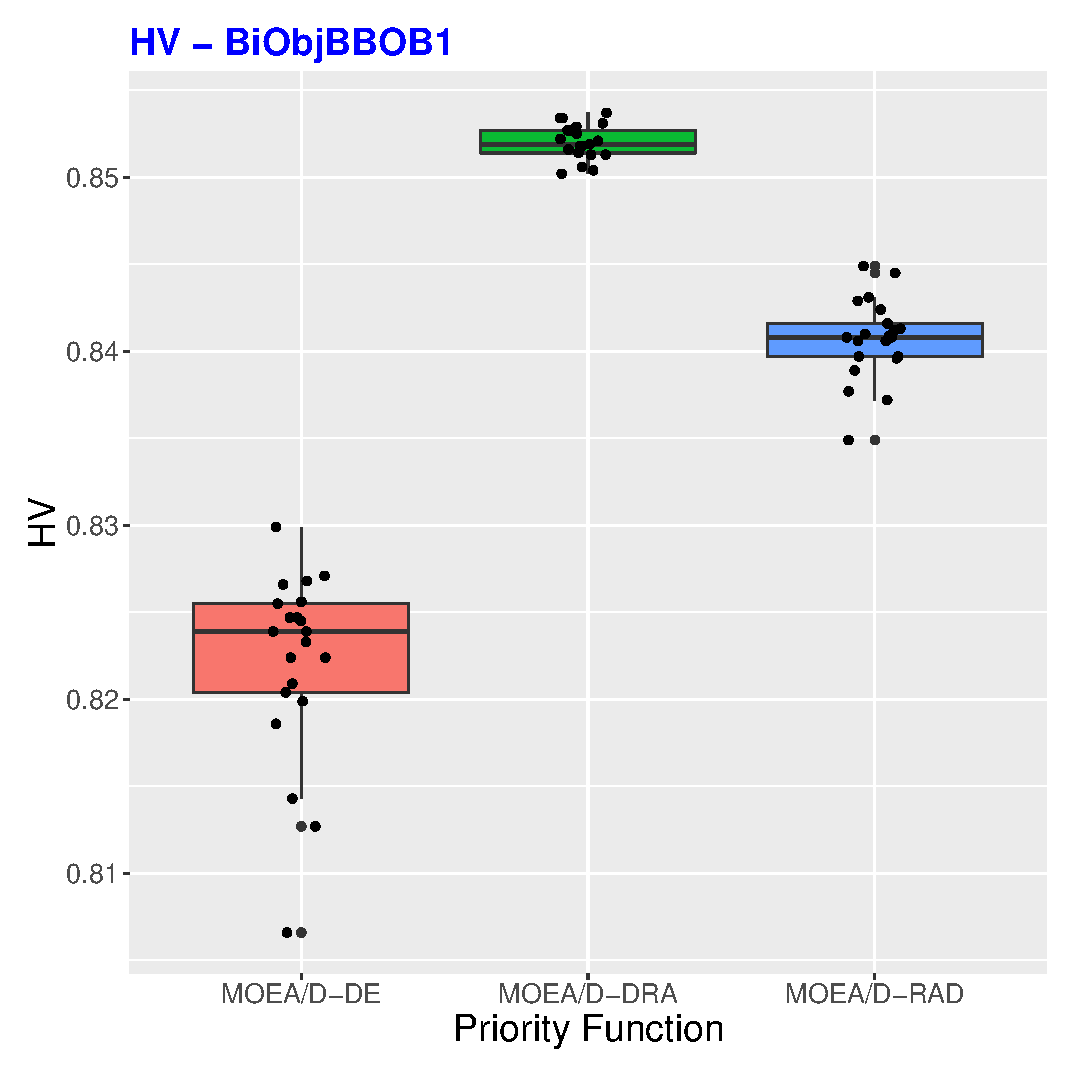
\includegraphics[width=1\textwidth, height=1\textwidth]{img/BiObjBBOB1_HV.eps}
		%	\caption{HV - UF3}
	\end{subfigure}
	\begin{subfigure}[b]{0.33\textwidth}
		\centering
		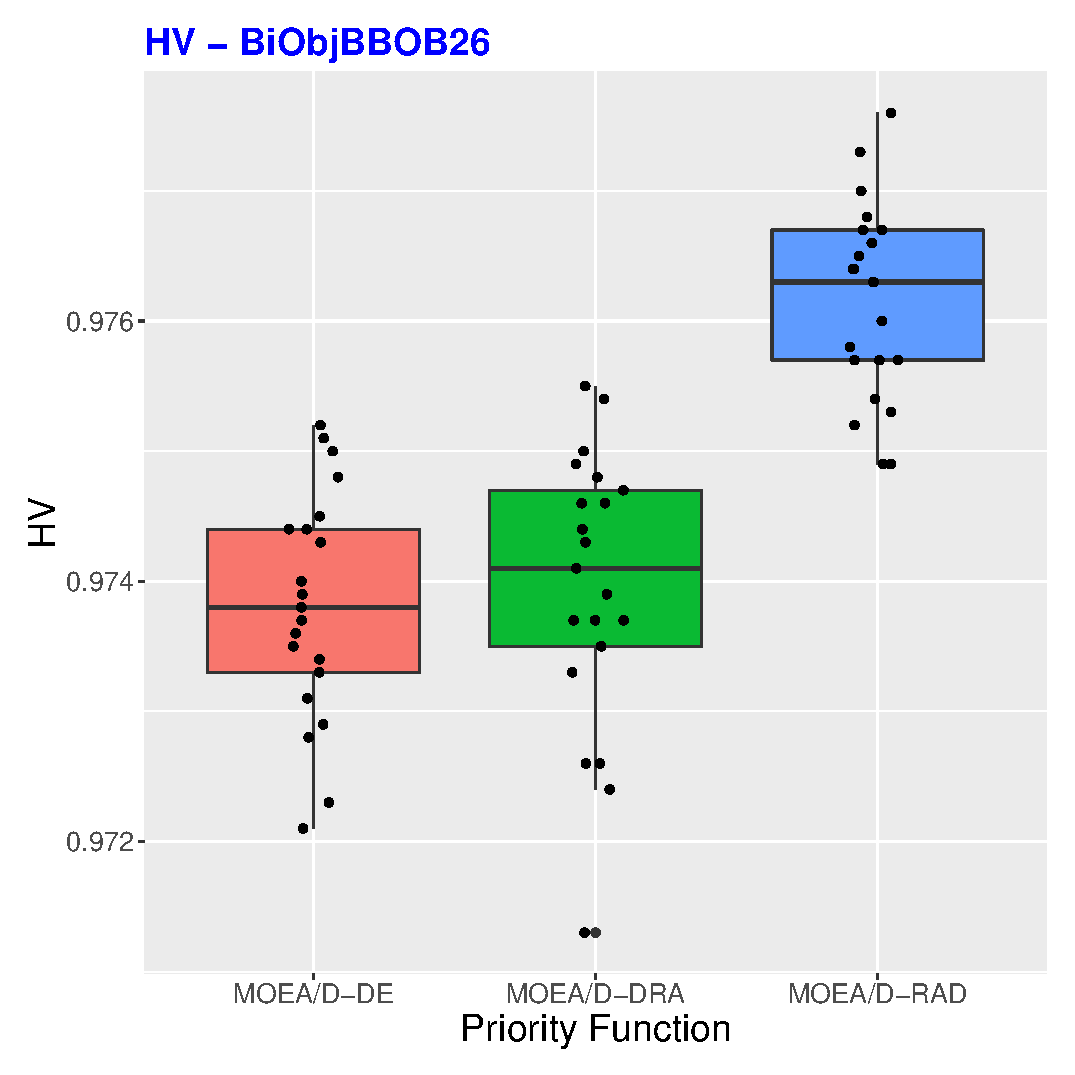
\includegraphics[width=1\textwidth, height=1\textwidth]{img/BiObjBBOB26_HV.eps}
		%	\caption{HV - UF8}
	\end{subfigure}
	\begin{subfigure}[b]{0.33\textwidth}
		\centering
		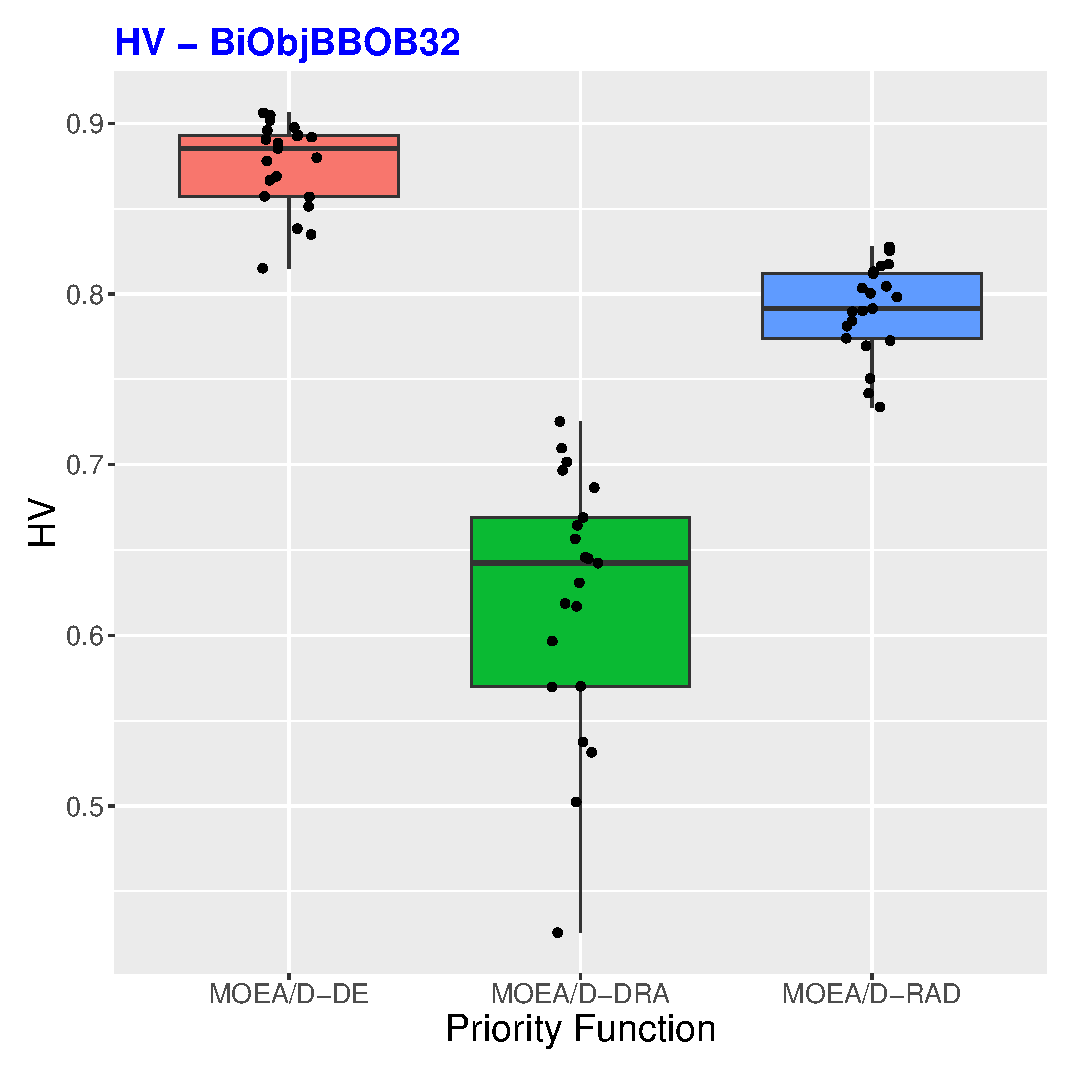
\includegraphics[width=1\textwidth, height=1\textwidth]{img/BiObjBBOB32_HV.eps}
		%	\caption{HV - DTLZ4}
	\end{subfigure}
	\caption{Box plot of HV values on  bbob-biobj-1,  bbob-biobj-26 and  bbob-biobj-32 (Higher values are better).}
	\label{HVS}
\end{figure*}

\begin{figure*}[!t]
	\centering
	%	\Large{Average performance on different tournament size - Gallagher's Gaussian 21-hi Peaks Function}
	\begin{subfigure}[b]{0.33\textwidth}
		\centering
		\includegraphics[width=1\textwidth, height=0.8\textwidth]{img/RA-DRA-26.eps}
	\end{subfigure}
	\begin{subfigure}[b]{0.33\textwidth}
		\centering
		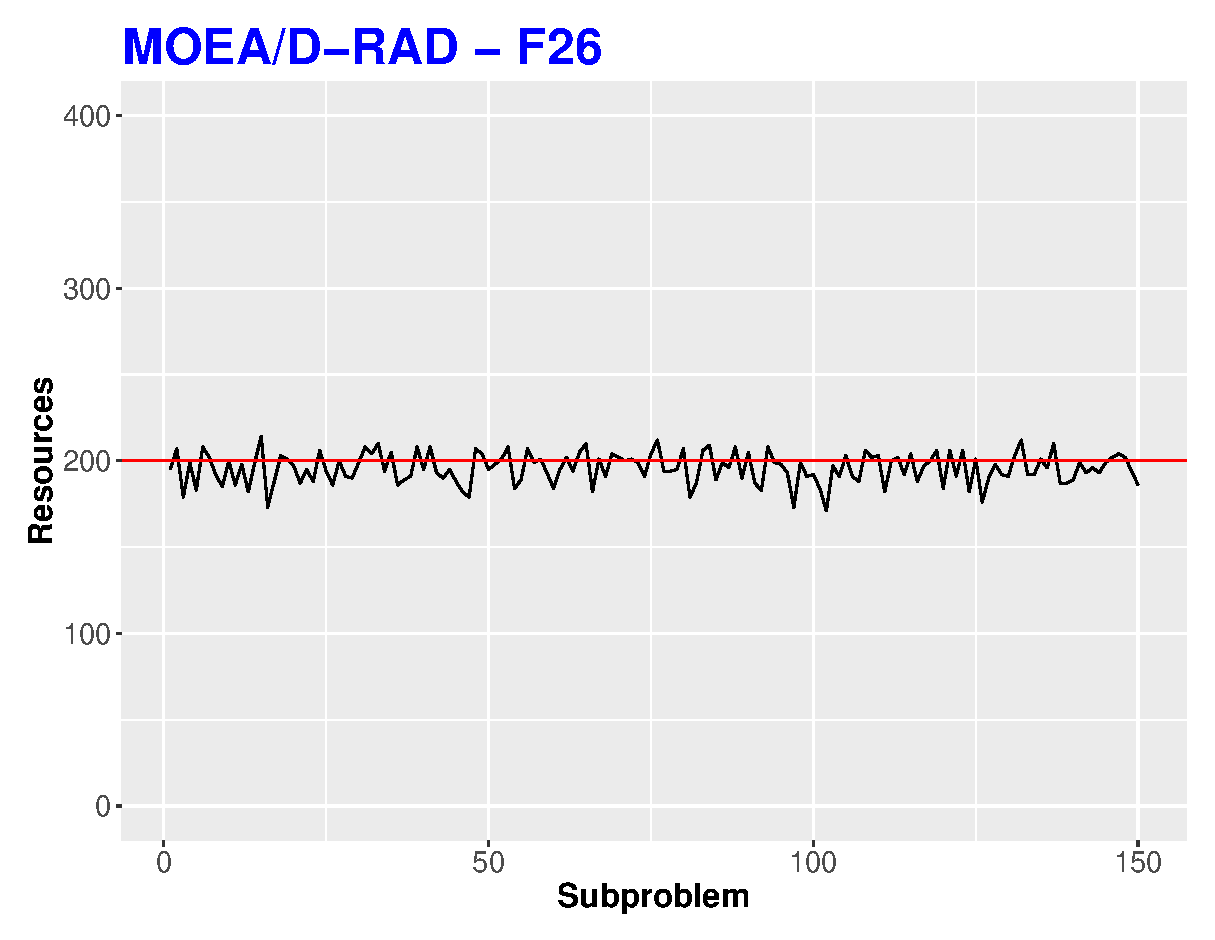
\includegraphics[width=1\textwidth, height=0.8\textwidth]{img/RA-RAD-26.eps}
	\end{subfigure}
	\caption{Resource Allocation by subproblem - The red line indicates the default amount of resource for each problem, i.e., with no priority function.}
	\label{RAs1}
\end{figure*}

\begin{figure*}[!t]
	\centering
	\begin{subfigure}[b]{0.33\textwidth}
		\centering
		\includegraphics[width=1\textwidth, height=0.8\textwidth]{img/RA-DRA-32.eps}
	\end{subfigure}
	\begin{subfigure}[b]{0.33\textwidth}
		\centering
		\includegraphics[width=1\textwidth, height=0.8\textwidth]{img/RA-RAD-32.eps}
	\end{subfigure}
	\caption{Resource Allocation by subproblem - The red line indicates the default amount of resource for each problem, i.e., with no priority function.}
	\label{RAs2}
\end{figure*}



\ref{HVS} shows the boxplots of the hypervolume values obtained by the three methods
on functions F26, F1 and F32 of bbob-biobj. F26 is an example of a moderate and
weakly structured function (group 9), where MOEA/D-RAD performed best. F1  is a
separable and separable function (group 1), where MOEA/D-DRA performed best, and
F32 is a moderate and multi-modal function (group 8), where MOEA/D-DE performed
.

\ref{stats} gives us a general view of these results over all functions and
function groups. In general, MOEA/D-RAD performed better than the other methods
(or second best) in terms of hypervolume. This ranking is reinforced by a
Pairwise Wilcoxon Rank Test over the entire experiment~(\ref{statistics}).

However, a post-hoc analysis of these results focusing on the function groups
suggests some interesting properties of the three methods. We observe that
MOEA/D-RAD was specially successful for function groups that included
moderate-conditioned or weakly-structured functions (groups 2, 5, 6, 7, 8, 9, 12 and
15, shaded in \ref{stats}), and performed slightly worse for groups including
multi-modal functions (groups 4, 8, 11, 13 and 14). In particular, we find it  very
interesting that MOEA/D-DE without priority performed better in the multi-modal
groups. This post-hoc analysis suggests a follow up experiment to confirm this
observations.

\subsection{Proportion of Non-dominated Solutions}

Another difference that we see among the algorithms  is the proportion of non
dominated solutions. The results on the~\ref{stats} indicate that MOEA/D-DRA
leads to the highest rate of non-dominated solutions in the final solution set,
followed by MOEA/D-RAD. In general, both substantially improve this proportion
over the results of MOEA/D-DE.  It seems that there is no relation between
hypervolume performance and the proportion of non-dominated solutions.


\subsection{Resource Allocation}


\ref{RAs1} and \ref{RAs2} illustrate the amount resource allocated by MOEA/D-DRA
and MOEA/D-RAD to each subproblem on problems F26 and F32. MOEA/D-DE is
not included since it does not perform resource allocation.

These figures show how the choice of priority function influences the
resource allocation. The resource allocation by MOEA/D-DRA is much more
adaptive to each problem, while the resource allocation done by
MOEA/D-RAD is more conservative and uniform.

However, even though the resource allocation behavior seen in these figures
may seem limited, it is clear from \ref{stats} that it has a deep impact on
the performance of the algorithm.

\input{51_tables.tex}

\section{Conclusion}

In this research, we propose a new algorithm for Resource Allocation in
Multi-Objective Optimization, MOEA/D-RAD. The performance of this algorithm is
studied on the bbob-biobj benchmark function set. This algorithm differs from
standard MOEA/D by the use of Resource Allocation techniques, which allocate
computational effort proportional to each subproblem's difficulty.

MOEA/D-RAD performs Resource Allocation using MRDL as a priority function based
on a geometrical perspective. In this sense, MOEA/D-RAD allocates computational
resources to different subproblems based on its contribution to the overall
diversity of the population.

We compared this new approach with MOEA/D-DRA, which is another
Resource Allocation strategy. MOEA/D-DRA allocates computational resources
based on the difference between parent and child solutions. We also compared
with MOEA/D-DE without Resource Allocation strategy.

The experimental results showed that MOEA/D-RAD performed well on several  of
the test problems. In particular, we observed that MOEA/D-RAD performed well in
functions that are moderate-conditioned and weakly-structured.  On the other
hand, MOEA/D-DRA showed the highest rate of non-dominated  solutions in the
final solution set.

In comparison with MOEA/D-DRA, the Resource Allocation by the proposed
MOEA/D-RAD was less extreme. This might explain why MOEA/D-RAD and MOEA/D-DE
were usually successful in similar functions, although MOEA/D-RAD always  had a
better proportion of non-dominated solutions, and often achieved better
hypervolume values than MOEA/D-DE. We understand that this shows that using the
MRDL function as the priority function achieved its goal of promoting diversity
in the solution set.

Overall, the findings of this work reinforce the need of Resource Allocation for
MOEA/D, and showcase particular types of functions where Resource Allocation
techniques would be most useful. The differences between MOEA/D-DRA and
MOEA/D-RAD also  suggests that the choice of priority function is a critical
component of Resource Allocation and that this choice needs to be informed by
the characteristics of the problem being solved.

Our results indicate that the MRDL priority function might be a reasonable
choice in problems where at least one objective is moderate-conditioned or
weakly structured. However, as this observation came from a post-hoc analysis,
further exploration is crucial to confirm this finding.

Other future works include further consideration into priority functions  (such
as objective-space and decision-space priority functions) as well as  Resource
Allocation and priority functions based on Archive techniques,  such as
MOEA/D-CRA~\cite{kang2018collaborative}.


\bibliography{sample}
\bibliographystyle{jpnsec}

%\bibliographystyle{IEEEtran}

%\bibliography{sample}
%\bibliographystyle{jpnsec}

%
%􏰂
%
%\begin{biography}
%\profile{m}{進化 太郎}{著者の略歴}{portrait}
%\end{biography}


%\appendix
%\section{Appendix}
%
%%% Biography %%%%%%%%%%%%%%%%%%%%%%%%%%%%%%%%%%%%%%%%%%%%%%%%%%%%%%%%%%%%%%%%%%


\end{document}
